\chapter{Experiments and Results}
\thispagestyle{plain}
\label {Experiments and Results}

In this chapter we discuss the datasets used and the experiment setup to test the column separation, column annotations and relation predictions. We also evaluate the framework as we explain the results from the various experiments performed on the datasets.


\section{Data Setup}
We use different sets of log files to test the framework. Primarily, we use two datasets viz., original log files and synthetically generated log files. Table~\ref{table:dataset_distribution} gives a general statistic about the tables in every datasets, total columns and average columns present in each table of the dataset.

\begin{table}[htbp]
\caption{Number of log files, total columns present and the average number of columns in each dataset}
\bigskip
\label{table:dataset_distribution}
\centering
\begin{center}
\def\arraystretch{1.8}
\begin{tabular}{|@{\hskip 1cm}c@{\hskip 1cm}|c|c|c|}
\hline
\textit{Dataset} & \textit{Tables} & \textit{Columns} & \textit{Average Columns}\\ 
\hline
Original & 11 & 78 & 7\\
\hline
Synthetic & 20 & 150 & 8\\ 
\hline
\end{tabular}
\end{center}
\end{table}

The Original dataset contains actual log files as obtained from various tools and services running in an operating system. This includes \textit{Linux} system services like syslog, kern, auth, etc. We also have log files from commonly used services like apache2, mongodb, sendmail, printers, etc.
\\

The Synthetic dataset has a set of artificially generated log files using some known columns. These columns are generally seen in log files like those present in the Original dataset. The synthetic log files were generated to test the framework against log files with unknown format and source.

To create these synthetic log files, we randomized the whole process. The number of columns in every log file was randomly chosen. Later, we arbitrarily selected the type of columns from the manually extracted superset of columns. While generating the columns we probabilistically added different column values to the selected columns. This was intended to simulate unpredictable nature of log files. Also, all the values added in the columns for a particular type were generated at random to ensure variation in length and other properties of the column.


\section{Tabulation}

In this experiment we tested the precision with which the log files are converted into tables with proper columns. The \textit{Tabulate} module of the framework, splits the log file to convert it into a table. This is a simple test where we have log files with the separable columns. We feed these log files to the \textit{Tabulate} module and get an output table with certain set of columns. We try and match all the output columns to the expected sample of columns. Thus, we not only check the number of columns separated we also check the exact boundaries of separation.

\begin{figure}[h]
	\centering
	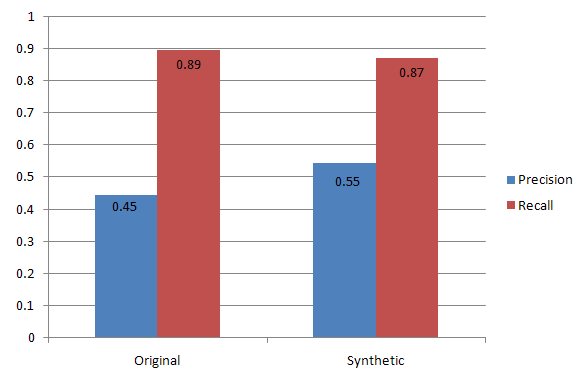
\includegraphics[width=\textwidth, height=0.5\textheight, keepaspectratio] {tabulate_precision_recall_1.png}
	\caption{Precision and Recall for Column Separation}
	\label{fig:tabulate_precision_recall_1}
\end{figure}

As discussed in previous chapter, we separate the log files using standard delimiters. Due to this, certain columns having multiple words but no surrounding characters, get separated as multiple columns. It has been observed in most of the cases, such descriptive columns with multiple words are found at the tail of the log entry. Thus, most of the initial columns are easily separated. Due to the said fact about log files, our framework can give out more columns than the expected number of columns. We also get a high recall as we do not expect those columns to be separated. While the recall is high, we observe a low precision. Due to the extraneous columns, which are not there in the original log files, we get a low precision compared to the recall. In Figure~\ref{fig:tabulate_precision_recall_1} we see that for both the datasets, we get a high recall and low precision.

We repeat this experiment with the same log files, but now we strip out the trailing textual part. In real life, we can find tools which can clean the log files and in this case strip the unwanted text. Figure~\ref{fig:tabulate_precision_recall_2} shows the precision and recall with the modified log files. Now, we see that both precision and recall are high for the datasets.

\begin{figure}[h]
	\centering
	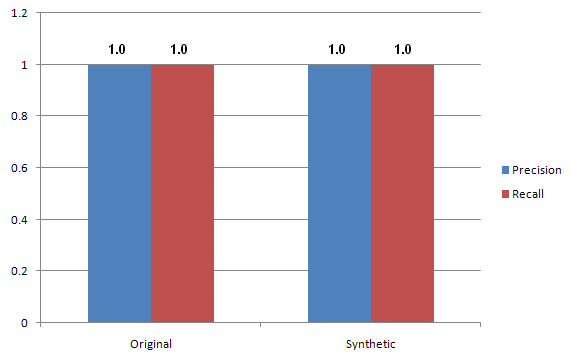
\includegraphics[width=\textwidth, height=0.5\textheight, keepaspectratio] {tabulate_precision_recall_2.png}
	\caption{Precision and Recall for Column Separation without Trailing Textual Data}
	\label{fig:tabulate_precision_recall_2}
\end{figure}

